% mn2esample.tex
%
% v2.1 released 22nd May 2002 (G. Hutton)
%
% The mnsample.tex file has been amended to highlight
% the proper use of LaTeX2e code with the class file
% and using natbib cross-referencing. These changes
% do not reflect the original paper by A. V. Raveendran.
%
% Previous versions of this sample document were
% compatible with the LaTeX 2.09 style file mn.sty
% v1.2 released 5th September 1994 (M. Reed)
% v1.1 released 18th July 1994
% v1.0 released 28th January 1994

\documentclass[useAMS,usenatbib]{mn2e}

% If your system does not have the AMS fonts version 2.0 installed, then
% remove the useAMS option.
%
% useAMS allows you to obtain upright Greek characters.
% e.g. \umu, \upi etc.  See the section on "Upright Greek characters" in
% this guide for further information.
%
% If you are using AMS 2.0 fonts, bold math letters/symbols are available
% at a larger range of sizes for NFSS release 1 and 2 (using \boldmath or
% preferably \bmath).
%
% The usenatbib command allows the use of Patrick Daly's natbib.sty for
% cross-referencing.
%
% If you wish to typeset the paper in Times font (if you do not have the
% PostScript Type 1 Computer Modern fonts you will need to do this to get
% smoother fonts in a PDF file) then uncomment the next line
% \usepackage{Times}

%%%%% AUTHORS - PLACE YOUR OWN MACROS HERE %%%%%
\usepackage{subfigure}
\usepackage{amsmath}	% Advanced maths commands
\usepackage{amssymb}	% Extra maths symbols
\usepackage{graphicx}

\newcommand{\bz}{\bmath{z}}
\newcommand{\bA}{\bmath{A}}
\newcommand{\bB}{\bmath{B}}
\newcommand{\bC}{\bmath{C}}
\newcommand{\bE}{\bmath{E}}
\newcommand{\bF}{\bmath{F}}
\newcommand{\bG}{\bmath{G}}
\newcommand{\br}{\bmath{r}}
\newcommand{\bg}{\bmath{g}}
\newcommand{\bd}{\bmath{d}}
\newcommand{\bv}{\bmath{v}}
\newcommand{\bn}{\bmath{n}}
\newcommand{\by}{\bmath{y}}
\newcommand{\bJ}{\bmath{J}}
\newcommand{\bD}{\bmath{D}}
\newcommand{\bH}{\bmath{H}}
\newcommand{\bN}{\bmath{N}}
\newcommand{\bM}{\bmath{M}}
\newcommand{\bI}{\bmath{I}}
\newcommand{\ba}{\bmath{a}}
\newcommand{\bb}{\bmath{b}}
\newcommand{\bzero}{\bmath{0}}
%\newcommand{\bvarrho}{\bmath{\varrho}}
%\newcommand{\bnu}{\bmath{\nu}}
%\newcommand{\bvarphi}{\bmath{\varphi}}
\newcommand{\conj}[1]{\overline{#1}}

%%%%%%%%%%%%%%%%%%%%%%%%%%%%%%%%%%%%%%%%%%%%%%%%

\title[Unknown]{TBD}
\author[A. V. Raveendran and A. N. Other]{A. V. Raveendran$^{1}$\thanks{E-mail:
email@address (AVR); otheremail@otheraddress (ANO)} and A. N.
Other$^{2}$\footnotemark[1]\thanks{This file has been amended to
highlight the proper use of \LaTeXe\ code with the class file.
These changes are for illustrative purposes and do not reflect the
original paper by A. V. Raveendran.}\\
$^{1}$Indian Institute of Astrophysics, Bangalore 560034, India\\
$^{2}$Building, Institute, Street Address, City, Code, Country}
\begin{document}

\date{Accepted 1988 December 15. Received 1988 December 14; in original form 1988 October 11}

\pagerange{\pageref{firstpage}--\pageref{lastpage}} \pubyear{2002}

\maketitle

\label{firstpage}

\begin{abstract}
TBD
\end{abstract}

\begin{keywords}
circumstellar matter -- infrared: stars.
\end{keywords}

\section{Introduction}

Main contributions of the paper:

\begin{enumerate}
 \item Present a general framework which unifies all the techniques developed so far showing they are all related (LINCAL, non-linear estimator, etc ...). They are all non-linear
 least-squares techniques, i.e. they either employ Gauss-Newton or the Levenberg-Marquardt algorithms. We have to start with LINCAL showing that it is GN, then we have to motivate 
 why we want to use Oleg's complex optimization framework.
 \item Use Oleg's complex optimization framework to re-derive the non-linear technique proposed by Marthi and Chengular. The novelty lies, in the fact that by using Oleg's
 framework we can find analytic expressions for the Jacobian, the Hessian and the Jacobian-residual product (which is not even the case for LINCAL). State that the algorithm is 
 effectively related to SteFCal and is eff an independent rediscovery of SteFCal and an extension of it into the redundant domain.
 \item Also we present the array geometry function to help us make the derivations from Marthi and Chengular easier to read and understand for a general layout.
 \item We also mention at this point that in Oleg's paper the question is raised is there a fast way of computing the exact inverse, we then present this new method, which is called
 conjugate gradient method. We discuss the algorithm and the two things which bound its execution time. Which is $kappa$ and $m$ (spectral condition number and its sparsity). Then
 we explore both of these parameters.
 \end{enumerate}
 
 **************
 FLOW OF PAPER
 **************
 
 \begin{enumerate}
 \item We need the definition of visibilities as in Liu. DEFINE SNR HERE ALREADY together maybe with the sigma value of the noise.
 \item Introduce the array geometery function.
 \item Write down logcal and lincal in matrix form... ?
 \item Short discussion of least squares and jacobian and hessian's. General GN and LM update rules.
 \item Introduce redundant calibration as a least squares problem. We will use this general fact to derive both popular methods.
 \item Propose a possible solution witch leads to lincal. Mention that this approach works as in this form the function is differentiable (a taylor expansion in the 
 parameters exists). Maybe mention that we can also divide the problem into real and imaginary etc...
 \item Show how this relates to lincal for example ---> show lincal is GN.
 \item Now introduce complex optimization ---> Main motivation for switching to the alternative framework is that the the differentials are very simplistic. We wish to show that
 we can derive the method of Chengular.
 \item Do the derivation of Chengular. 
 \item Brief discussion abouth Chengular and SteFCal and Complex Optimization. Here I show that in Oleg's paper he re-derives an algorithm called SteFCal. Stefcal works
 on the basis of alternating direction implicit method. The first signs of achieving a similar algorithm already appeared in Stefan's conference paper in which the alternating
 idea was first proposed. Then I mention Chegular re-derives the expression by using partial derivatives and extends it to redundant. One could also have used the linear alternating
 approach. In an attempt to merge the terminology that has independently develop in the general calibration and redundant calibration literature and to emphasize the close
 relationship between Stefcal and the approach derived by I will use the label Redunandat SteFCal (R-Stefcal) to refer to the NLS method proposed by ... Lastly we mention that similarly
 to how Oleg re-derived stefcal in, we have achieved the same approach.
 \item Faster Exact inverse. A question that Oleg poses in his paper is, does there exist a faster way to take the exact inverse of JhJ? One that is almost linear, and
 implies that we can therefore implement the full LM algorithm. The aim here is of course to reduce the number of iterations that are required to converge by using the 
 full inverse instead which would hopefully provide enough of a speedup to compensate for the more expensive full-inverse. The algorithm we propose is the conjugate 
 gradient method.
 \item We give the images of the HESSIAN of both lincal and the complex method (number of terms). So we can mention that both are sparse and contain diagonal entries that 
 are more significant than the off-diagonal entries. What linear inversion approach can take advantage of both these phenomenon. One such technique is 
 cg. 
 \item Briefly discuss CG and how its computationally bounded by its condition number and its sparsity (how does the diagonal play a role).
 \item Simulation description
 \item Will CG improve things?
 \item Now first discuss the condition
 number of the Hessian before and after pre-conditioning (pre-codnitioning can only be applied if a good inverse of a matrix is known, if it is known then it can improve 
 the spectral condition number of a matrix. We present here the kappa and iteration number graphs for the HEXAGONAL layout. Although the
 \item Now we discuss the sparsity results. 
 \item Provide a table that theoretical compares R-StEFCal and SPARC.
 \item Number of outerloop iterations. 
 \item Timing results.
 \item Accuracy results.
 \item Maybe some freq simulations.
 \end{enumerate}
 
 We
 
 \section{Visibilities}
The observed visibility $d_{pq}$ measured by the baseline formed by antenna $p$ and $q$ can be described as

\begin{equation}
\label{eq:vis_definition}
d_{pq} = g_{p}\conj{g}_{q}y_{pq} + n_{pq},
\end{equation}
where $g_{p}$ and $g_{q}$ are the direction independent gains associated with antenna $p$ and $q$, $y_{pq}$ denotes the true visibility that baseline $pq$ measured
and $n_{pq}$ is the thermal noise component. Conjugation is denoted by $\conj{(*)}$. During the course of an actual observation the true value of $g_p$, $g_q$ and $y_{pq}$ are unknown and are the quantities which infact have 
to be estimated.

The real and imaginary components of the thermal noise is normally distributed with a mean of zero and a standard deviation that is equal to [NB - are the real and imaginary parts defined with same sigma?]  
\begin{equation}
\sigma = \frac{\sqrt{2}k_{B}T_{\textrm{sys}}}{A\eta\sqrt{\Delta \nu \tau}}, 
\end{equation}
where $k_B$ is Boltzmann's constant, $T_{\textrm{sys}}$ is equal to the system temperature, $A$ is the effective collecting area of each element in the array, $\eta$ is a dimensionless
efficiency factor, $\Delta \nu$ is the observational bandwidth and $\tau$ is the integration time per visibility. 

\subsection{Redundant Array Geometry Function}
If an array is redundant then its redundant baselines sample the exact same visibilites in the $uv$-plane, i.e. if baseline $pq$ and $rs$ are redundant then $y_{pq} = y_{rs}$. We can
therefore also use the following useful indexing strategy: we can use singular redundant baseline indexes instead of composite antenna pairs to label the true observed visibilities. 

Let $\phi_{ij}:\mathbb{N}^2\rightarrow\mathbb{N}^+$ be the function that maps composite antenna pairs to the unique redundant baseline indexes of an array. We refer to this function 
as the redundant array geometry function in this paper. This mapping is not symmetric as 
$\phi_{ij} = 0$ if $i>j$. We can also define the following symmetric variant of $\phi_{ij}$:
\begin{equation}
\zeta_{ij} = 
\begin{cases}
\phi_{ij}~\textrm{if}~i\leq j\\
\phi_{ji}~\textrm{if}~i>j
\end{cases}.
\end{equation} 
It is possible to construct a simple analytic expression for $\zeta_{ij}$ when our array is in an east-west regular configuration, namely $\zeta_{ij} = |j-i|$. 
It becomes increasingly more difficult to construct analytic expressions of $\zeta_{ij}$ for other more complicated array layouts. The empirically constructed symmetric geometry
functions of three different redundant layouts are depicted in Fig.~\ref{fig:geometry_function}. We denote the range of $\zeta_{ij}$ with $\mathcal{R}(\zeta_{ij})$. The maximal element 
that $\zeta_{ij}$ can ascertain is denoted by $L$ and can be construed as the maximal number of unique redundant baselines which can be formed for a given 
array layout. Alternatively, we can interpret the symmetric geometry functions 
in Fig.~\ref{fig:geometry_function} as matrices. In this alternative paradigm, $\zeta_{ij}$ denotes a matrix entry instead. The dimension of these so called geometry 
matrices are $N\times N$, where $N$ denotes the number of antennas in the array. 

\begin{figure*}
\centering
\subfigure[Hexagonal layout]
{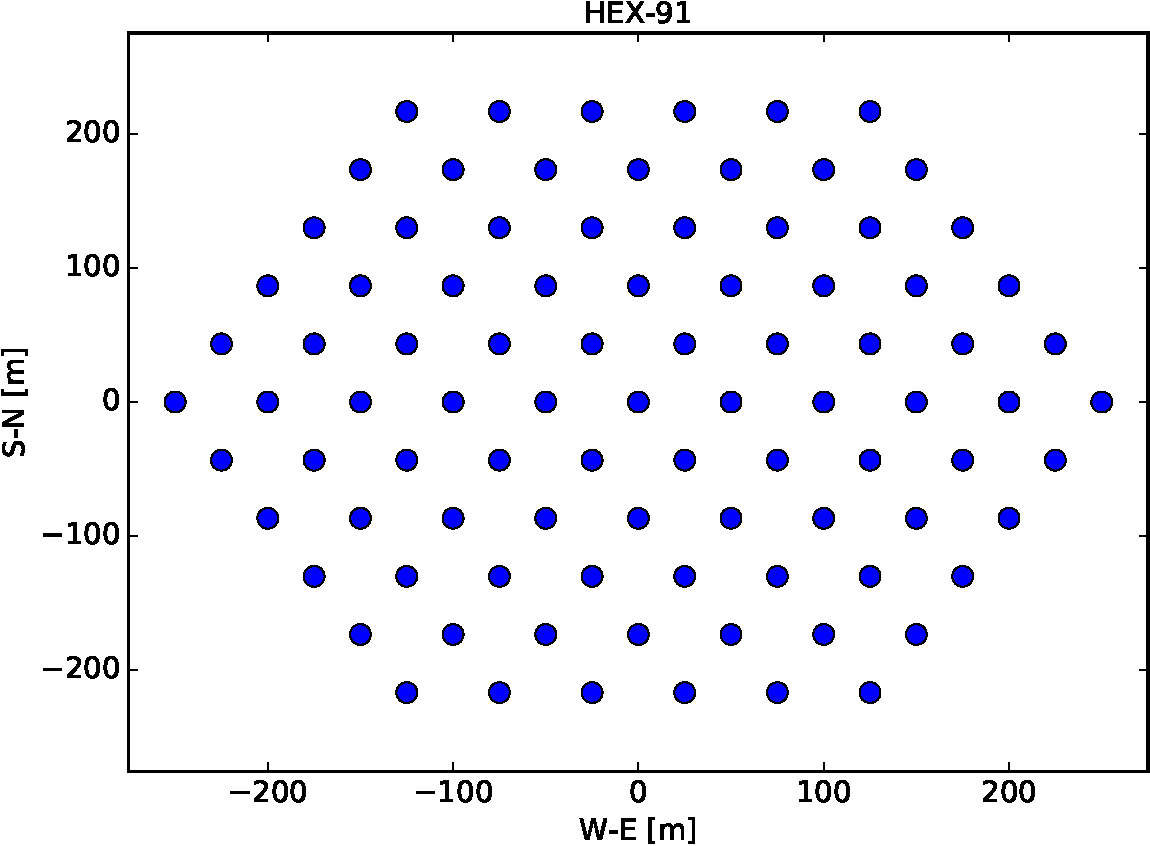
\includegraphics[width=0.33\textwidth]{./HEX_lay.pdf}\label{fig:HEX_lay}}
\subfigure[Square layout]
{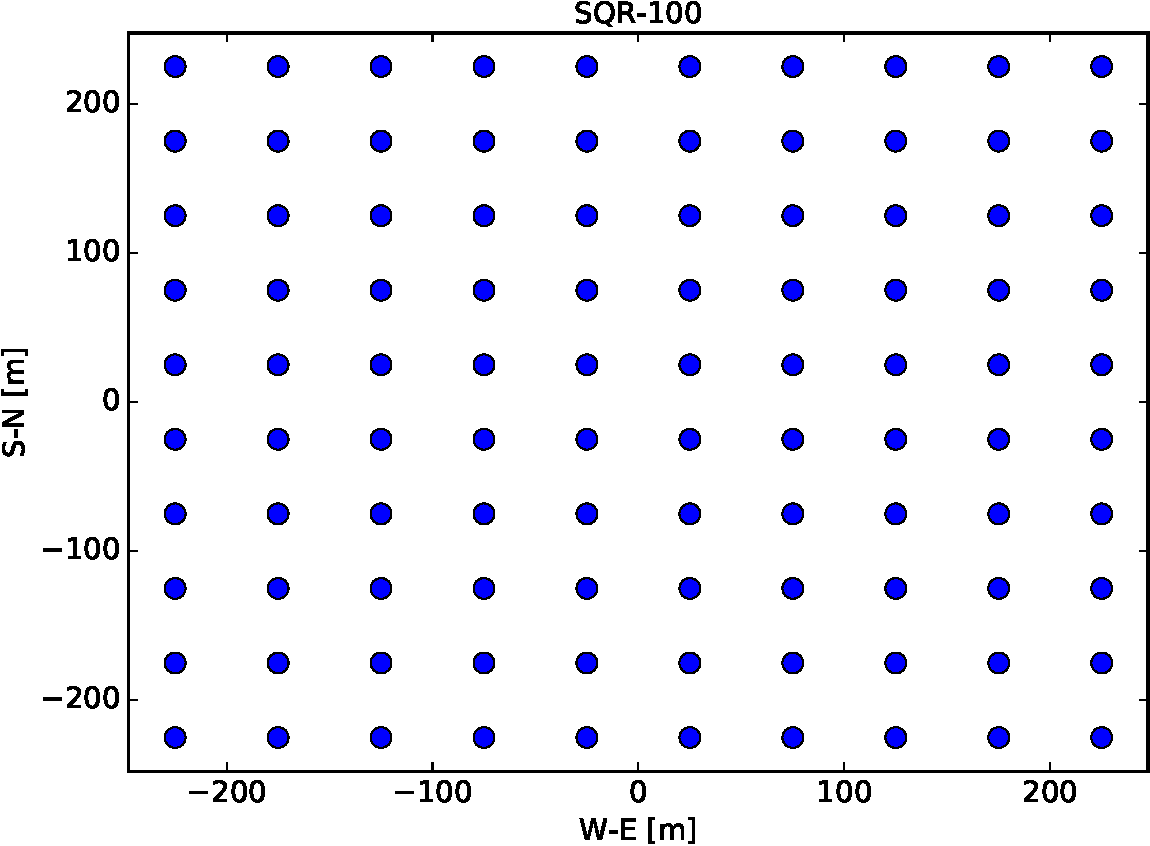
\includegraphics[width=0.33\textwidth]{./SQR_lay.pdf}\label{fig:SQR_lay}}
\subfigure[Regular east-west layout]
{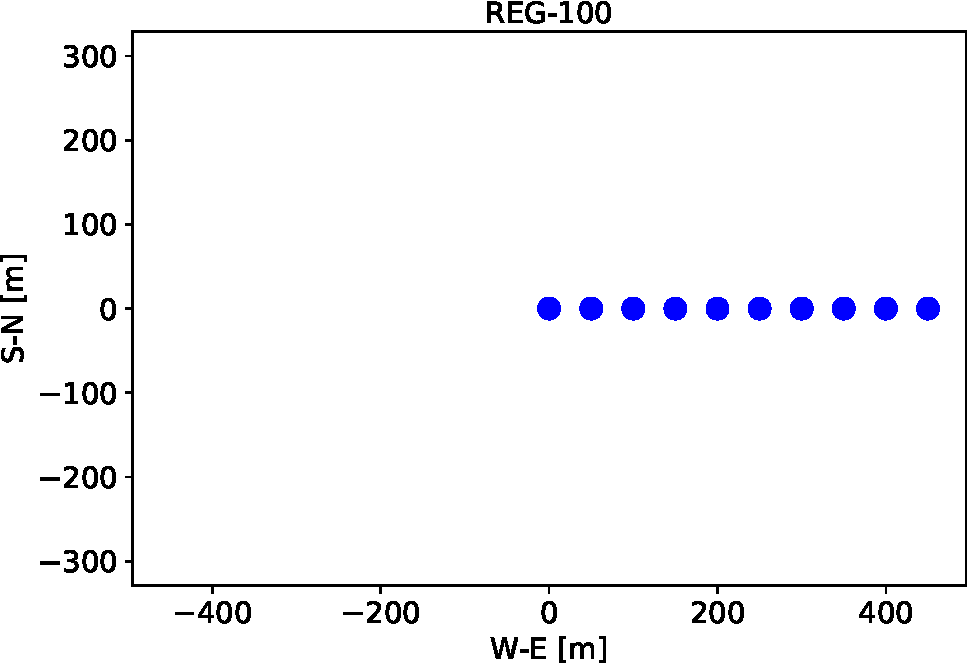
\includegraphics[width=0.33\textwidth]{./REG_lay.pdf}\label{fig:REG_lay}}

\subfigure[Hexagonal: $\zeta_{pq}$]
{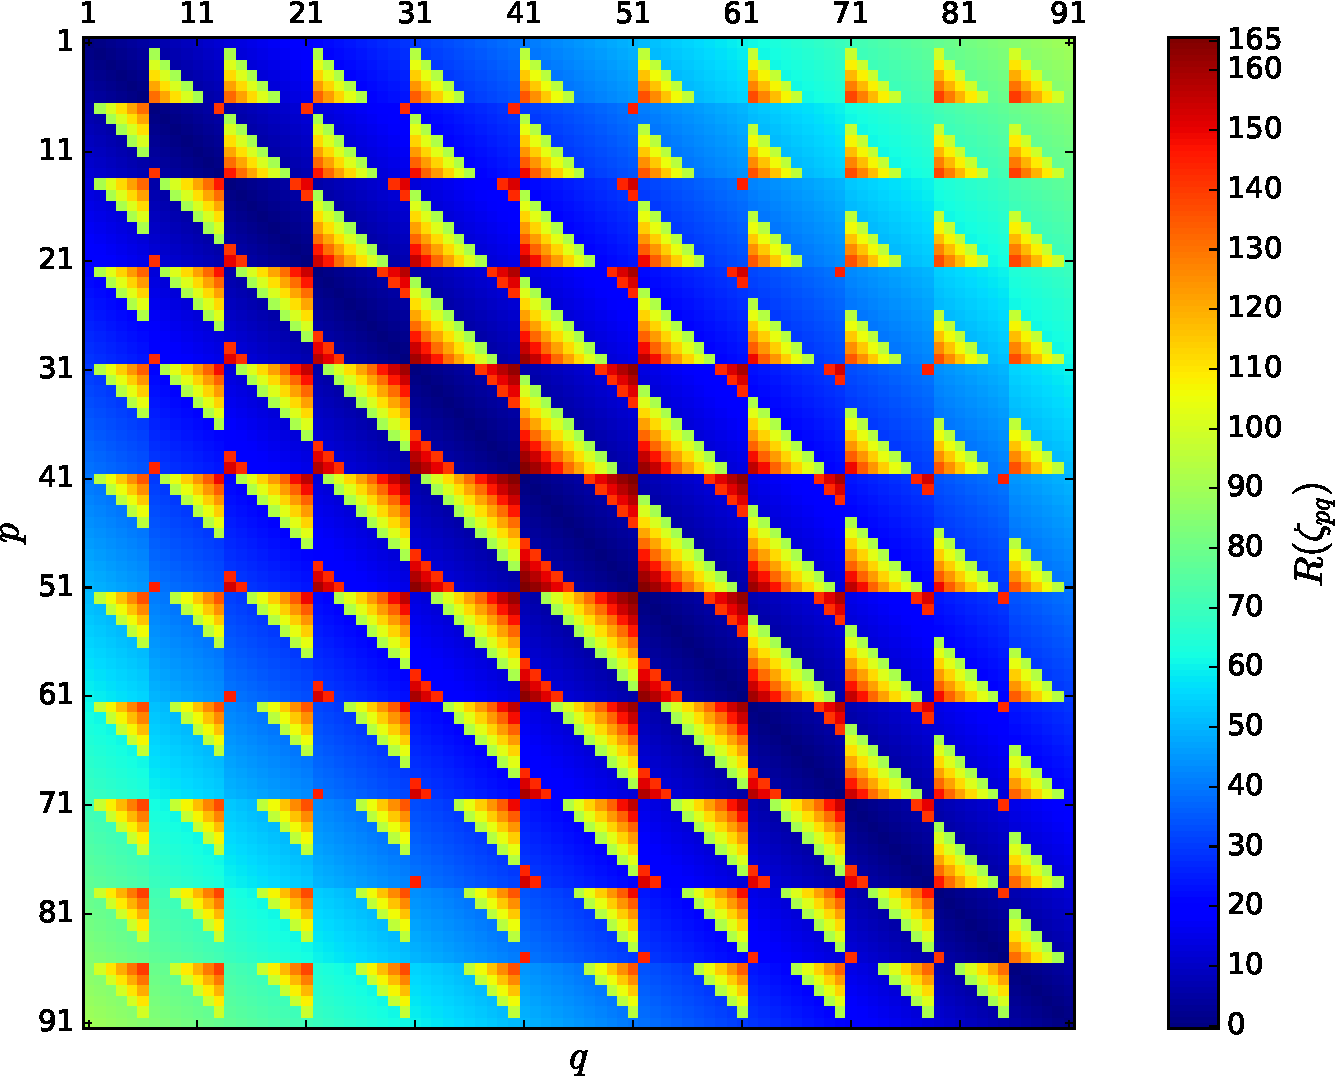
\includegraphics[width=0.33\textwidth]{./HEX_phi.pdf}\label{fig:HEX_phi}}
\subfigure[Square: $\zeta_{pq}$]
{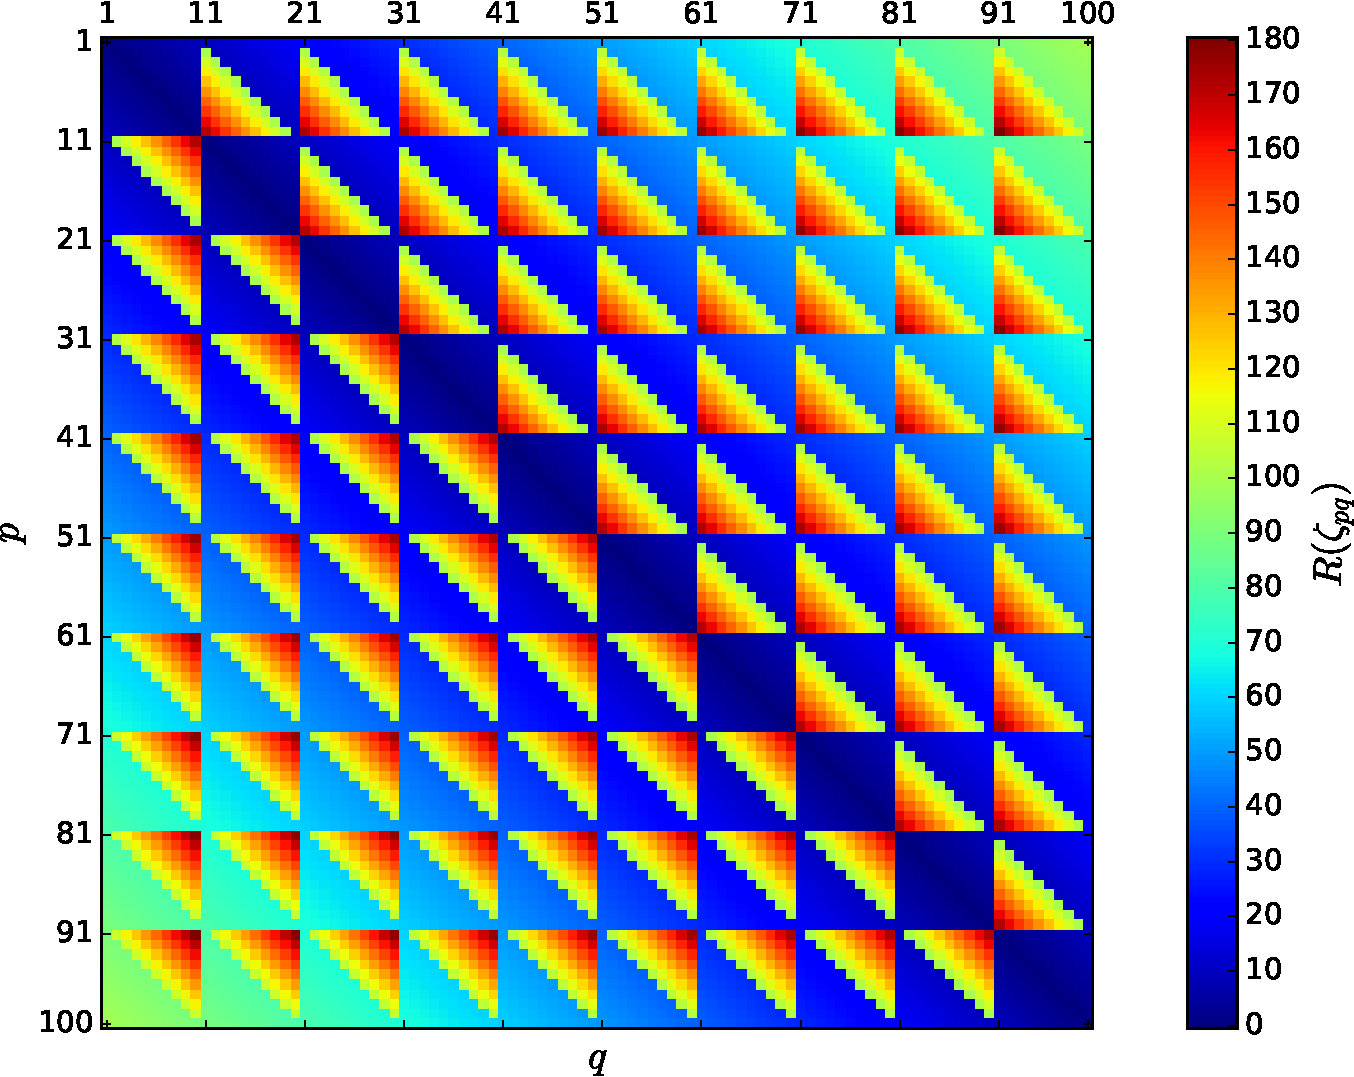
\includegraphics[width=0.33\textwidth]{./SQR_phi.pdf}\label{fig:SQR_phi}}
\subfigure[Regular east-west: $\zeta_{pq}$]
{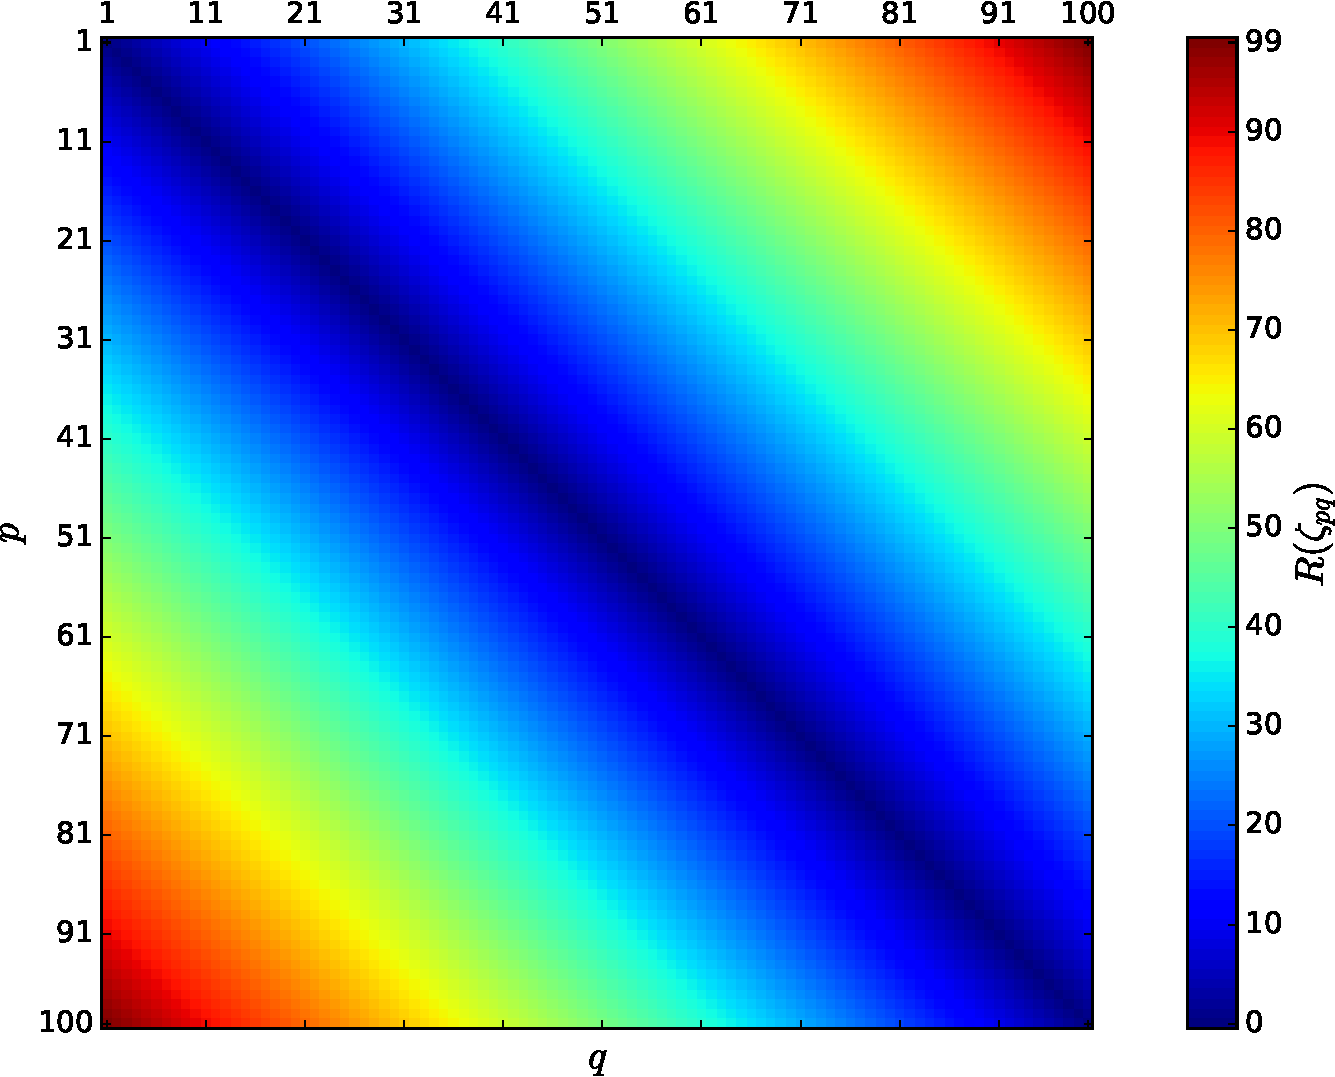
\includegraphics[width=0.33\textwidth]{./REG_phi.pdf}\label{fig:REG_phi}}
\caption{In the top panel we have three different redundant antenna layouts, namely a hexagonal (left), square (middle) and a regular east-west (right) layout. 
In the bottom panel we have the respective symmetric redundancy geometry functions for the layouts on the top panel. We used 91 antennas
to construct the the hexagonal layout, while a 100 antennas where used in the square and east-west layouts. The maximal amount of redundant baselines that can be formed for 
the hexagonal, square and east-west layouts in the top panel are 165, 180 and 99 baselines respectively.\label{fig:geometry_function}}
\end{figure*}

If the function $\phi_{ij}$ is known and one is given one of the two antenna indexes that together form a redundant baseline as well as the redundant baseline index itself then it is possible 
to calculate the unknown antenna index. This can be computed via the following two expressions:
\begin{equation}
\xi_{ij} = 
\begin{cases}
p~\textrm{if}~\exists! ~ p \in \mathbb{N} ~ s.t. ~(\phi_{pi} = j)\\
0~\textrm{otherwise}
\end{cases},
\end{equation}
and
\begin{equation}
\psi_{ij} = 
\begin{cases}
q~\textrm{if}~\exists! ~ q \in \mathbb{N} ~ s.t. ~(\phi_{iq} = j)\\
0~\textrm{otherwise}
\end{cases}
\end{equation}
We use $\xi_{ij}$ to retrieve the first antenna index of the composite antenna pair associated with a particular baseline, if the index of the first antenna in the composite antenna pair and the unique redundant baseline index are known, while we use $\psi_{ij}$ to obtain 
a similar result; the second antenna index of the composite antenna pair. \textbf{NB::} I still need to plot $\zeta_{ij}$ for different antenna layouts.

\subsection{Signal-to-noise Ratio}
If the array is redundant and the function $\phi_{ij}$ is known we can rewrite Eq.~\eqref{eq:vis_definition} as
\begin{equation}
\label{eq:vis_red}
d_{pq} = g_{p}\conj{g}_{q}y_{\phi_{pq}} + n_{pq}.
\end{equation}
Eq.~\eqref{eq:vis_red} can also be expressed in the following vector form 
\begin{equation}
\bd = \bv + \bn, 
\end{equation}
where 
\begin{align}
 \left [ \bd \right]_{\alpha_{pq}} &= d_{pq}, & \left [ \bv \right ]_{\alpha_{pq}} &= g_p y_{\phi_{pq}} \conj{g}_q\nonumber\\
 \left [ \bn \right ]_{\alpha_{pq}} &= n_{pq}. &  &\label{eq:vec_definitions}
\end{align}
In Eq.~\eqref{eq:vec_definitions}, the size of the three vectors are equal to $B$ (i.e. $p<q$), which denotes the number of baselines in the array. Moreover,
\begin{equation}
\alpha_{pq} =
\begin{cases}
(q-p) + (p-1)\left (N-\frac{1}{2}p \right ) & \textrm{if}~p<q\\
B + (p-q) + (q-1)\left (N-\frac{1}{2}q \right )) & \textrm{if}~p>q\\
%B+q + \frac{1}{2}(p-1)(p-2) & \textrm{if}~p>q\\
0 & \textrm{otherwise}
\end{cases}.
\end{equation}
The easiest way to construct the vectors in Eq.~\ref{eq:vec_definitions} is to enumerate through the composite indexes $pq$ in the following order $12, 13,\cdots,1N,23,\cdots$.
For each composite index we then compute the right hand side of the appropriate vector element definition which we then need to assign to the 
correct vector position. The correct position is calculated with $\alpha_{pq}$. Using the aforementioned order, however, allows you to fill the vector in numerical order, i.e. $12,13,\cdots,1N,23,\cdots \xrightarrow{\alpha_{pq}} 1,2,3,\cdots,B$.  


We will be using the following SNR (signal-to-noise ratio) definition in this paper  
\begin{equation}
\textrm{SNR} = \frac{<\bv\odot\conj{\bv}>_{t,pq}}{<\bn\odot\conj{\bn}>_{t,pq}}, 
\end{equation}
where $<*>_{t,pq}$ denotes averaging over time and baselines and $\odot$ denotes the Hadamard product. The definition we use here is based on the SNR definitions used in \citet{Liu2010} and \citet{Marthi2014}.

\subsection{LOGCAL}
NEED BETTER INTRO\\
One of the best known algorithms that is currently used to perform redundant calibration involves the use of logarithms. If we ignore the noise term then we can 
rewrite Eq.~\eqref{eq:vis_red} as
\begin{eqnarray}
\ln |d_{pq}| &=& \ln |g_p| + \ln |g_q| + \ln |y_{\phi_{pq}}| \label{eq:logcal_amp}\\
\angle d_{pq} &=& \angle g_p - \angle g_q + \angle \phi_{pq} \label{eq:logcal_phase}
\end{eqnarray}

We can easily express Eq.~\eqref{eq:logcal_amp} with the following linear system
\begin{equation}
\widetilde{\bd} = \bA\widetilde{\bz}, 
\end{equation}
where
\begin{equation}
\left [ \widetilde{\bd}\right ]_{\alpha_{pq}} = \ln |d_{pq}|,\nonumber\\ 
\end{equation}
\begin{equation}
\widetilde{\bz} = \begin{bmatrix}
                  \ln | \bg |\\
                  \ln | \by |
                  \end{bmatrix},
\end{equation}
with $\bg = [g_1,g_2,\cdots,g_N]^T$ and $\by = [y_1,y_2,\cdots,y_L]^T$.

Furthermore,
\begin{equation}
\label{eq:A}
\bA = \begin{bmatrix}
       \bA_1 & \bA_2
      \end{bmatrix}
\end{equation}
and
\begin{equation}
\left [ \bA_1 \right ]_{\alpha_{pq},j} = \delta^j_p\vee\delta^j_q,  ~~~ \left [ \bA_2 \right ]_{\alpha_{pq},j} = \delta_{\phi_{pq}}^j. 
\end{equation}

The dimensions of $\bA_1$ and $\bA_2$ are $B\times N$ and $B\times L$.
Moreover, $\vee$ denotes the logical or operator and
\begin{equation}
\delta_y^x  = \begin{cases}
          1 & \textrm{if}~x=y\\
          0 & \textrm{otherwise}
         \end{cases}.
\end{equation}
A similar linear system can be constructed for Eq.~\eqref{eq:logcal_phase}.\\

NEED TO ROUND OF HERE STILL 

\subsection{LINCAL}
Assume that $\eta_p,\eta_q,\widetilde{\eta}_{\phi_{pq}},\varphi_p,\varphi_q$ and $\widetilde{\varphi}_{\phi_{pq}}$ are real valued variables.
Substituting $g_p$ with $e^{\eta_p - i \varphi_p}$, $g_q$ with $e^{\eta_q - i \varphi_q}$ and $y_{\phi_{pq}}$ with $e^{\eta_{\widetilde{\phi}_{pq}}- i \widetilde{\varphi}_{\phi_{pq}}}$ in Eq.~\eqref{eq:vis_red} results in  
\begin{equation}
\label{eq:lincal}
d_{pq} =  e^{\eta_p - i \varphi_p} e^{\widetilde{\eta}_{\phi_{pq}}- i \widetilde{\varphi}_{\phi_{pq}}} e^{\eta_q + i \varphi_q} + n_{pq}.
\end{equation}

A possible approach one can use to solve the unknowns in Eq.~\eqref{eq:lincal} is to write down the Taylor expansion of the first term of the right hand side of Eq.~\eqref{eq:lincal} around some 
initial fiducial guess of $\eta_p,\eta_q,\widetilde{\eta}_{\phi_{pq}},\varphi_p,\varphi_q$ and $\widetilde{\varphi}_{\phi_{pq}}$, which we denote with 
$\eta_p^0,\eta_q^0,\widetilde{\eta}_{\phi_{pq}}^0,\varphi_p^0,\varphi_q^0$ and $\widetilde{\varphi}_{\phi_{pq}}^0$, and then to solve the perturbations from this 
initial guess that minimize the difference between the right and left hand side of Eq.~\eqref{eq:lincal}. Once the perturbation values 
have been computed it is trivial to obtain an estimate of $g_i$, $g_j$ and $y_{\phi_{ij}}$. 

If we Taylor expand the first term on the right hand side of Eq.~\eqref{eq:lincal} around a fiducial initial guess we obtain
\begin{equation}
\label{eq:taylor_expansion}
d_{pq} = v_{pq}^0[1+\Delta \eta_p + \Delta \eta_q + i \varphi_p - i \Delta \varphi_q + \Delta \widetilde{\eta}_{\phi_{pq}} + i\Delta \widetilde{\eta}_{\phi_{pq}}] + n_{pq}, 
\end{equation}
where
\begin{equation}
v_{pq}^0 = e^{\eta_p^0 - i \varphi_p^0} e^{\widetilde{\eta}_{\phi_{pq}}^0 - i \widetilde{\varphi}_{\phi_{pq}}^0} e^{\eta_q^0 + i \varphi_q^0}, 
\end{equation}
and $\eta_p^0,\eta_q^0,\widetilde{\eta}_{\phi_{pq}}^0,\varphi_p^0,\varphi_q^0$ and $\widetilde{\varphi}_{\phi_{pq}}^0$ respectively denote the initial guess for $\eta_p,\eta_q,\widetilde{\eta}_{\phi_{pq}},\varphi_p,\varphi_q$ and $\widetilde{\varphi}_{\phi_{pq}}$.
Eq.~\eqref{eq:taylor_expansion} can be used to construct the following linear system
\begin{equation}
\breve{\br} = \bJ\Delta\widehat{\bz}, 
\end{equation}
where 
\begin{equation}
\left [ \breve{\br} \right ]_{\alpha_{pq}} = d_{pq}-v_{pq}^0, 
\end{equation}
\begin{equation}
\label{eq:jac_lincal}
\bJ = \begin{bmatrix}
      \bN & \bM\\
      \conj{\bN} & \conj{\bM}
      \end{bmatrix}
\end{equation}
and
\begin{equation}
\Delta\widehat{\bz} = 
\begin{bmatrix}
\Delta \bmath{\eta} \\
\Delta \bmath{\varphi} \\
\Delta \widetilde{\bmath{\eta}} \\
\Delta \widetilde{\bmath{\varphi}},
\end{bmatrix}
\end{equation}
with
\begin{align}
 \Delta \bmath{\eta} &= [\Delta \eta_1,\Delta \eta_2,\cdots \Delta \eta_N]^T\nonumber\\
 \Delta \bmath{\varphi} &= [\Delta \varphi_1,\Delta \varphi_2,\cdots \Delta \varphi_N]^T\nonumber\\
 \Delta \widetilde{\bmath{\eta}} &= [\Delta \widetilde{\eta_1},\Delta \widetilde{\eta_2},\cdots \Delta \widetilde{\eta_N}]^T\nonumber\\
 \Delta \widetilde{\bmath{\varphi}} &= [\Delta \widetilde{\varphi_1},\Delta \widetilde{\varphi_2},\cdots \Delta \widetilde{\varphi_N}]^T.
\end{align}

Furthermore, 
\begin{equation}
\bN = \begin{bmatrix}
      \bN_1 & \bN_2 
      \end{bmatrix},
\end{equation}
with 
\begin{align}
[\bN_1]_{\alpha_{pq},j} &= \frac{\partial v_{pq}}{\partial \eta_j} {\bigg |}_{\widehat{\bz}=\widehat{\bz}^0}\\
&= (\delta_{p}^{j}\vee\delta_{q}^{j}) v_{pq}^0,
\end{align}
and
\begin{align}
 [\bN_2]_{\alpha_{pq},j} &= \frac{\partial v_{pq}}{\partial \varphi_j} {\bigg |}_{\widehat{\bz}=\widehat{\bz}^0}\\
 &= (-1)^{\delta_{q}^{j}}i(\delta_{p}^{j}\vee\delta_{q}^{j}) v_{pq}^0. 
\end{align}

Moreover,
\begin{equation}
\bM = \begin{bmatrix}
      \bM_1 & \bM_2 
      \end{bmatrix},
\end{equation}
with
\begin{align}
[\bM_1]_{\alpha_{pq},j} &= \frac{\partial v_{pq}}{\partial \widetilde{\eta}_j} {\bigg |}_{\widehat{\bz}=\widehat{\bz}^0}\\
&=  \delta_{\phi_{pq}}^{j} v_{pq}^0,
\end{align}
and
\begin{align}
[\bM_2]_{\alpha_{pq},j} &= \frac{\partial v_{pq}}{\partial \widetilde{\varphi}_j} {\bigg |}_{\widehat{\bz}=\widehat{\bz}^0}\\
&= i\delta_{\phi_{pq}}^{j} v_{pq}^0,
\end{align}

STILL NEEDS LOTS OF WORK.

\section{Least Squares}
Redundant calibration can be achieved by solving the following optimization problem
\begin{equation}
\label{eq:red_least_squares}
\min_{\bz} \|\br\| = \min_{\bz} \|\bd - \bv(\bz)\|, 
\end{equation}
where $\bz = [\bg,\by]^T$. Eq.~\eqref{eq:red_least_squares} is a nonlinear least squares problem.

The most standard way of solving a general least squares problem is to use a gradient type of minimization algorithm whose main purpose is to find the model parameters that 
minimizes the difference between the observed and model data. In this paper we will be focusing on the following gradient minimization algorithms: Gauss-Newton and Levenberg-Marquardt (cite LM here). For the redundant calibration problem in Eq.~\eqref{eq:red_least_squares} $\bd$, which is the corrupted observed visibilities, is the observed data,
while $\bv$, which is the predicted visibilities, represents the model data.\footnote{In this paper we use the same symbol to denote predicted visibilities and true observed visibilities as it
is trivial to distinguish which one is implied from the context.}   

The gradient based minimization algorithms that are generally used to solve least squares problems generally require the model $\bv$ to be differentiable
towards each model parameter. When the least squares problem is complex, which is the case for Eq.~\eqref{eq:red_least_squares}, it becomes less straightforward to apply these gradient based minimization methods. The reason being,
many complex functions are not analytic (no Taylor expansion around a fiducial point exists) and therefore not differentiable if the classic notion of differentiation is used. For instance if the 
classical definition of differentiation is used then $\frac{\partial z}{\partial \conj{z}}$, where $z \in \mathbb{C}$, does not exist.

The only way to circumvent the differentiability conundrum that plaques complex least square problems is to recast our complex optimization problem in such a way that $\bv$ becomes analytic in its argument.
The standard way of achieving this is to divide the complex optimization problem into its real and imaginary parts and then to solve for the real and imaginary parts of the parameters separately.

Recently Kreutz-Delgado and Sorber proposed an alternative strategy, which involves the use of Wirtinger calculus (Wirtinger 1927). The Wirtinger derivatives 
are defined to be 
\begin{align}
\frac{\partial}{\partial z} &= \frac{1}{2}\left ( \frac{\partial}{\partial x} -  i \frac{\partial}{\partial y} \right ),&\frac{\partial}{\partial \conj{z}} &= \frac{1}{2}\left ( \frac{\partial}{\partial x} +  i \frac{\partial}{\partial y} \right ). 
\end{align}
Using the above definitions we can now easily compute the following:
\begin{align}
\frac{\partial z}{\partial z} & = 1, & \frac{\partial \conj{z}}{\partial z}&=0, & \frac{\partial z}{\partial \conj{z}} & = 0, & \frac{\partial \conj{z}}{\partial \conj{z}}&=1.
\end{align}

\citet{Smirnov2015} recently proposed to use this Wirtinger framework instead of the classic real and imaginary approach to perform normal calibration. We will now show
that the Wirtinger framework can also be applied to redundant calibration. Analogous to \cite{Smirnov2015}, we recast Eq.~\eqref{eq:red_least_squares} to 
\begin{equation}
\label{eq:red_least_squares_complex}
\min_{\breve{\bz}} \|\breve{\br}\| = \min_{\breve{\bz}} \|\breve{\bd} - \breve{\bv}(\breve{\bz})\|, 
\end{equation}
where $\breve{\bz} = [\bz,\conj{\bz}]^T$, $\breve{\bd} = [\bd,\conj{\bd}]^T$, $\breve{\bv} = [\bv,\conj{\bv}]$. Eq.~\eqref{eq:red_least_squares_complex} is the augmented counterpart of Eq.~\eqref{eq:red_least_squares}.
If we use the Wirtinger derivative instead of the classic notion of a derivative to define the gradient operator then 
$\bv$ becomes analytic in $\bz$ and $\conj{\bz}$ as a whole. The fact that $\bv$ is now analytic in its argument has the immediate consequence that it becomes possible to use the Gauss-Newton
and the Levenberg-Marquardt algorithm to solve Eq.~\eqref{eq:red_least_squares_complex} \citep{Smirnov2015}.

STILL NEEDS LOADS OF WORK. REFERENCES.

\subsection{Complex GN and LM}
In this section we discuss how we can use the GN and LM algorithms to solve Eq.~\eqref{eq:red_least_squares_complex} (i.e. estimate $\breve{\bz}$). The complex Jacobian is defined to be
\begin{equation}
\label{eq:Jacobian}
\bJ = \begin{bmatrix}
       \bJ & \bJ^*\\
       \conj{\bJ}^* & \conj{\bJ} 
      \end{bmatrix},
\end{equation}
where 
\begin{align}
\bJ &= \frac{\partial \bv}{\partial \bz}, & \bJ^* &= \frac{\partial \bv}{\partial \conj{\bz}}. 
\end{align}
In Eq.~\eqref{eq:Jacobian}, $\frac{\partial}{\partial \bz}$ and $\frac{\partial}{\partial \conj{\bz}}$ respectively denote the cogradient operator and the conjugate cogradient operator (cite Sorber).
The GN update step is now defined as:
\begin{equation}
\label{eq:GN_update}
 \Delta \breve{\bz} = (\bJ^H\bJ)^{-1}\bJ^H\breve{\br}.
\end{equation}
The LM update rule is very similar, the major difference being a damping factor $\lambda$ is introduced:
\begin{equation}
\Delta \breve{\bz} = (\bJ^H\bJ + \lambda\bD)^{-1}\bJ^H\breve{\br},
\end{equation}
where $\bD=\bI\odot\bJ^H\bJ$. 
NEED TO MENTION THE SILENT INDEX $k$ AND HOW THE UPDATE RULE IS ITERATIVE. ALSO MENTION THAT $\lambda$ IMPROVES THE CONVERGENCE PROPERTIES. WE WILL REFER TO $\bJ^H\bJ$ AS THE 
HESSIAN.

\subsection{Redundant Jacobian and Hessian}
If we apply the definition in Eq.~\eqref{eq:Jacobian} to Eq.~\eqref{eq:red_least_squares_complex} we obtain the following analytic result:
\begin{equation}
\label{eq:Jacobian_red}
\bJ = \begin{bmatrix}
       \bM & \bN\\
       \conj{\bN} & \conj{\bM}
      \end{bmatrix},
\end{equation}
where
\begin{equation}
\bM =\begin{bmatrix}
      \bM_1 & \bM_2
     \end{bmatrix},
\end{equation}
and 
\begin{equation}
\bN = \begin{bmatrix}
       \bN_1 & \bzero
      \end{bmatrix}.
\end{equation}
Moreover,
\begin{align}
\left [ \bM_1 \right ]_{\alpha_{pq},j} &= y_{\phi_{pq}}\conj{g}_q\delta_p^j, & \left [ \bM_2 \right ]_{\alpha_{pq},j} &= g_p\conj{g}_q\delta_{\phi_{pq}}^j 
\end{align}
and
\begin{equation}
\left [ \bN_1 \right ]_{\alpha_{pq},j} = g_py_{\phi_{pq}}\delta^j_q. 
\end{equation}

It is now trivial to compute the Hessian $\bJ^H\bJ$ by using Eq.~\eqref{eq:Jacobian_red}. If we substitute Eq.~\eqref{eq:Jacobian_red} into $\bJ^H\bJ$
we obtain 
\begin{equation}
\bH = \bJ^H\bJ = 
\begin{bmatrix}
\bA & \bB\\
\conj{\bB} & \conj{\bA}
\end{bmatrix},
\end{equation}
where

\begin{align}
\bA &= \begin{bmatrix} \bC & \bD\\ \bD^H & \bE \end{bmatrix}, & \bB &= \begin{bmatrix} \bF & \bG\\ \bG^T & \bzero \end{bmatrix},
\end{align}

\begin{equation}
[\bC]_{ij} = 
\begin{cases}
 \sum_{k \neq i} \left | g_k \right |^2 \left | y_{\zeta_{ik}} \right |^2 & \textrm{if} ~ i=j\\
 0 & \textrm{otherwise}
\end{cases},
\end{equation}
\begin{equation}
[\bD]_{ij} = 
\begin{cases}
 g_i \conj{y}_j  \left | g_{\psi_{ij}} \right |^2  & \textrm{if} ~ \psi_{ij}\neq0\\
 0 & \textrm{otherwise}
\end{cases},
\end{equation}

\begin{equation}
[\bE]_{ij} = 
\begin{cases}
 \sum_{pq \in \mathcal{PQ}_i} \left | g_p \right |^2 \left | g_q \right |^2  & \textrm{if} ~ i=j\\
 0 & \textrm{otherwise}
\end{cases},
\end{equation}
\begin{equation}
[\bF]_{ij} = 
\begin{cases}
 g_i g_j  \left | y_{\zeta_{ij}} \right |^2  & \textrm{if} ~ i \neq j\\
 0 & \textrm{otherwise}
\end{cases},
\end{equation}
and
\begin{equation}
[\boldsymbol{G}]_{ij} = 
\begin{cases}
 g_i y_j  \left | g_{\xi_{ij}} \right |^2  & \textrm{if} ~ \xi_{ij}\neq0\\
 0 & \textrm{otherwise}
\end{cases}.
\end{equation}

Moreover, $(*)^T$ denotes matrix transposition and

\begin{equation}
\mathcal{PQ}_i = \left\{pq\in\mathbb{N}^2|(\phi_{pq} = i) \right\}.
\end{equation}

HAVE TO MAKE SURE I DEFINE ALL THE MATH SYMBOLS THAT I USE. IF NOT HERE THEN EARLIER....

Furthermore, substituting Eq.~\eqref{eq:Jacobian_red} into $\bJ^H\breve{\br}$ results in
\begin{equation}
\bJ^H\breve{\br} = \begin{bmatrix}
                   \ba & \bb & \conj{\ba} & \conj{\bb}\\
                   \end{bmatrix}^T,
\end{equation}
where
\begin{align}
\left [ \ba \right ]_i &= \sum_{k\neq i} g_k \widetilde{y}_{ik}r_{ik},  & \left [ \bb \right ]_i &= \sum_{pq\in\mathcal{PQ}_i}\conj{g}_p g_q r_{pq},
\end{align}
and
\begin{equation}
\widetilde{y}_{ik} = 
\begin{cases}
\conj{y}_{\zeta_{ik}} & \textrm{if}~k > i\\
y_{\zeta_{ik}} & \textrm{otherwise}
\end{cases}.
\end{equation}

HAVE TO RECHECK THE ABOVE EQUATIONS DIRECTLY FROM THE CODE.

HAVE TO STATE WHETHER COLUMN OR ROW VECTOR.


% \begin{equation}
% \boldsymbol{J}^H\breve{\boldsymbol{d}} = 
% \begin{bmatrix}
% \sum_{k\neq i } g_k x_{ik}d_{ik}\\
% \sum_{pq \in \mathcal{I}_j} \conj{g}_p g_q d_{pq}\\
% \downarrow^{*}
% \end{bmatrix}
% \begin{matrix}% matrix for right braces 
% \coolrightbrace{\sum g_k x_{\zeta_{ik}}d_{ik}}{i = 1\cdots N}\\
% \coolrightbrace{\sum \conj{g}_p g_q d_{pq}}{j = 1\cdots L}\\
% \vphantom{\downarrow^{*}}
% \end{matrix}
% \end{equation}



\subsection{Simplifying GN}

The following identities,
\begin{align}
\label{eq:identities}
\frac{1}{3}\bJ\breve{\bz} &= \breve{\bv}, & \bJ^H\breve{\bv} &= (\bI\odot\bH)\breve{\bz} 
\end{align}
are trivially established by mechanically showing that the left hand side of each identity in Eq.~\eqref{eq:identities} is equal to its right hand side.

The first identity in Eq.~\eqref{eq:identities} can now be used to simplify Eq.~\eqref{eq:GN_update} as follows:
\begin{align}
\Delta \breve{\bz} &= (\bJ^H\bJ)^{-1}\bJ^H(\breve{\bd}-\breve{\bv})\\
&=(\bJ^H\bJ)^{-1}\bJ^H\breve{\bd}-\frac{1}{3}\breve{\bz}
\end{align}

STILL NEED TO ADD z k+1 EXPRESSION.

\subsection{GN and LINCAL}
As we mentioned at the start of this section, the Wirtinger framework is not the only way in which we can ensure that $\bv$ is analytic in its argument. We could also 
have divided the problem in Eq ... into its real and imaginary components and then solver for the real and imaginary parts of the parameters separately. There is a third way
of dealing with the issue. We can split the problem in Eq into its phase and amplitude components and then solve for the amplitude and phase of the parameters separately.
This can be achieved by first rewriting Eq. as

\begin{equation}
\label{eq:red_least_squares_lincal}
\min_{\bmath{\varrho}} \|\breve{\br}\| = \min_{\bmath{\varrho}} \|\breve{\bd} - \breve{\bv}(\bmath{\varrho})\|, 
\end{equation}
where $\bmath{\varrho} = \left [\bmath{\eta},\bmath{\varphi},\widetilde{\bmath{\eta}}, \widetilde{\bmath{\varphi}}\right ]^T$. The Jacobian associated with 
Eq.~\eqref{eq:red_least_squares_lincal} is equal to the Eq xxx in the LINCAL section.
We have therefore shown that doing one iteration of LINCAL is equivalent to a basic GN update step; the GN update step was just re-derived in the Appendix from first principles.
An easy why of improving the convergence properties of LINCAL would be to simply add the LM damping factor to the basic LINCAL update step. 

\subsection{LM and StEFCal}



















cite the complex paper has proposed to extend the problem into [RW HERE NEED TO STATE BETTER] its conjugate domain and then to solve for the parameters and there complex conjugates. This can be accomplished
if we introduce Wirtinger derivatives. (I have to look into how to write this better).

The solution to Eq. can now be obtained by using a gradient type of minimization algorithm, like GN and LM. 

The GN update rule is given by\\

GN UPDATE RULE


% fiducial initial guess 
% 
% The following partial derivatives are now easily computed
% 
% \begin{eqnarray}
% \frac{c_{ij}}{\partial \eta_p} &=& y_{i-j} e^{\eta_p - i \varphi_p} e^{\eta_q - i \varphi_q}\\ 
% \frac{c_{ij}}{\partial \varphi_p} &=&  -i y_{i-j} e^{\eta_p - i \varphi_p} e^{\eta_q - i \varphi_q}\\
% \frac{c_{ij}}{\partial \eta_q} &=& y_{i-j} e^{\eta_p - i \varphi_p} e^{\eta_q - i \varphi_q}\\ 
% \frac{c_{ij}}{\partial \varphi_q} &=&  i y_{i-j} e^{\eta_p - i \varphi_p} e^{\eta_q - i \varphi_q}\\
% \frac{y_{i-j}}{\partial \varphi_q} &=&  e^{\eta_p - i \varphi_p} e^{\eta_q - i \varphi_q}
% \end{eqnarray}
% 
% 
% The Wirtinger derivative is used in the last equation.
% 
% \begin{eqnarray}
% c_{ij} &\approx& c_{ij}^0 + \Delta \eta_p(y_{i-j}^0 e^{\eta_p^0 - i \varphi_p^0} e^{\eta_q^0 - i \varphi_q^0}) + \Delta \eta_q(y_{i-j}^0 e^{\eta_p^0 - i \varphi_p^0} e^{\eta_q^0 - i \varphi_q^0})\\
% && -i\Delta\varphi_p (y_{i-j}^0e^{\eta_p^0 - i \varphi_p^0} e^{\eta_q^0 - i \varphi_q^0}) +i\Delta\varphi_q (y_{i-j}^0e^{\eta_p^0 - i \varphi_p^0} e^{\eta_q^0 - i \varphi_q^0})\\
% && y_{i-j}^1(y_{i-j}^0e^{\eta_p^0 - i \varphi_p^0} e^{\eta_q^0 - i \varphi_q^0})\\
% &\approx&  c_{ij}^0 + e^{\eta_p^0 - i \varphi_p^0} e^{\eta_q^0 - i \varphi_q^0}(y_{i-j}^1 + y_{i-j}^0( \Delta \eta_p+ \Delta \eta_q - i\Delta\varphi_p + i\Delta\varphi_p))
% \end{eqnarray}
% 
% \begin{equation}
% \label{eq:residual}
% r_{ij} = \delta_{ij} = c_{ij}-c_{ij}^0 = e^{\eta_p^0 - i \varphi_p^0} e^{\eta_q^0 - i \varphi_q^0}(y_{i-j}^1 + y_{i-j}^0( \Delta \eta_p+ \Delta \eta_q - i\Delta\varphi_p + i\Delta\varphi_p)) 
% \end{equation}
% 
% Eq.~\ref{eq:residual} allows us to construct the following linear system:
% 
% \begin{equation}
% \boldsymbol{J}[\boldsymbol{\Delta \eta},\boldsymbol{\Delta \varphi},\boldsymbol{\Delta y}]^T = \boldsymbol{r}, 
% \end{equation}
% 
% where $\boldsymbol{J}$ is equal to 
% \begin{equation}
% \boldsymbol{J} = \bigg [\overbrace{\frac{c_{pq}}{\partial \eta_p}}^{i= 1\cdots N},~\overbrace{\frac{c_{pq}}{\partial \varphi_p}}^{i= 1\cdots N},~\overbrace{\frac{c_{pq}}{\partial y_{t}}}^{t=1\cdots r_s} \bigg ] \bigg \} [pq] = 1\cdots N_{\textrm{b}} (p<q) 
% \end{equation}
% or
% \begin{equation}
% \boldsymbol{J} = \bigg [\frac{c_{pq}}{\partial \boldsymbol{\eta}},~\frac{c_{pq}}{\partial \boldsymbol{\varphi}},~\frac{c_{pq}}{\partial \boldsymbol{y}} \bigg ] \bigg \} [pq] = 1\cdots N_{\textrm{b}} (p<q). 
% \end{equation}
% 
% The last column is again a Wirtinger derivative.
% 
% Which means we can obtain the least-squares estimate as follows:
% 
% \begin{equation}
% [\boldsymbol{\Delta \eta},\boldsymbol{\Delta \varphi},\boldsymbol{\Delta y}]^T = [\boldsymbol{J}^H\boldsymbol{J}]^{-1}\boldsymbol{J}^H\boldsymbol{r}.
% \end{equation}




\bibliographystyle{mn2e}
\bibliography{paper}

\label{lastpage}

\end{document}
